\pagina{Resultados de las pruebas del 13 de noviembre de 2026}
La sesión del 13 de noviembre contiene \textbf{24 intentos}, registrados entre las 15:56:25 y las 16:03:26. Todos utilizan \texttt{buffalo\_l} con vida \texttt{ambas}. Se mantienen separados de los 45 intentos de octubre porque son sesiones y condiciones distintas. Los resultados siguientes proceden de las etiquetas del archivo; hace falta revisar su correspondencia con el protocolo antes de atribuir cada error al algoritmo.

\subsection{Resumen de decisiones y tiempos}
\begin{center}\small\singlespacing
\begin{tabular}{P{2.7cm}rrrrrrrr}\toprule Condición & $n$ & Aciertos & \% & FR & FA & Media & Mediana & Máx. \\ \midrule
Foto en celular & 8 & 7 & 87,5 & 0 & 1 & 715,4 & 222,8 & 4100,7 \\
Luz normal & 16 & 4 & 25,0 & 11 & 1 & 3013,4 & 255,1 & 12021,2 \\
\bottomrule\end{tabular}
\end{center}
\tablenote{Tiempos en milisegundos. FR = falsos rechazos; FA = falsas aceptaciones, incluyendo aceptación con identidad distinta de la esperada. Fuente: \texttt{pruebas-2026-11-13.csv}. El resumen de análisis se incluye en los anexos CSV.}

Hay \textbf{11 aciertos en 24 intentos} (45,8\,\%). En luz normal, el archivo contiene 16 intentos que debían aceptarse: cuatro aceptaciones con identidad correcta, once decisiones de rechazo y una aceptación con otra identidad. Los cuatro intentos de s01 incluyen dos aciertos; los doce de s03 incluyen dos. La condición foto en celular reúne ocho intentos de s01: siete rechazos y una aceptación etiquetada como incorrecta.

\subsection{Casos que requieren revisión}
\begin{itemize}
\item \textbf{Foto aceptada, 16:00:10.} El archivo etiqueta el caso como \texttt{foto\_celular}, esperado rechazo, pero registra aceptación de s01 con similitud 0,7808, vida pasiva 1,00 y paralaje 0,26/0,26. El tiempo es 4100,7 ms. Se debe comprobar qué se presentó y reproducir la condición; no se omite este caso por haber siete rechazos correctos.
\item \textbf{Identidad distinta, 16:02:00.} El sujeto esperado es s03 y se registra aceptación como s04, similitud 0,7947, vida pasiva 1,00, paralaje 0,20/0,24 y 12021,2 ms. Dos capturas posteriores conservan esta decisión en pantalla; documentan el mismo resultado, no dos falsas aceptaciones adicionales.
\item \textbf{Rechazos de casos de aceptación.} Se registran fallos de giro a derecha e izquierda, rostro cortado y ocho rechazos de identidad con el detalle vacío. El CSV no permite fijar la causa de esos ocho casos. Conviene revisar etiquetas, vectores registrados, encuadre y configuración antes de repetir las pruebas.
\end{itemize}

Las dos FA no deben dividirse entre un único denominador: la aceptación en foto es 1/8 de los casos de rechazo; la confusión es 1/16 de los casos de aceptación. FR es 11/16 (68,75\,\%). Las medias y medianas incluyen rechazos tempranos, de modo que una mediana breve no implica que el acceso completo sea rápido.

\pagina{Bitácora de intentos y archivos CSV anexos}
Se conserva cada registro de noviembre sin corregir identidades ni etiquetas. La tabla resume sus campos principales; los CSV entregados mantienen también tecnología, resultado esperado, similitud y detalle. Luz normal tiene resultado esperado de aceptación; foto, de rechazo.
\begin{center}\small\singlespacing
\begin{tabular}{rlclllrr}\toprule N.º & Hora & Sujeto & Condición & Resultado & Identidad & ms & OK \\ \midrule
1 & 15:56:25 & s01 & Luz normal & Rechazo vida & s01 & 7206,3 & 0 \\
2 & 15:58:23 & s01 & Luz normal & Rechazo vida & s01 & 225,3 & 0 \\
3 & 15:58:33 & s01 & Luz normal & Acepta & s01 & 7164,1 & 1 \\
4 & 15:58:42 & s01 & Luz normal & Acepta & s01 & 3423,0 & 1 \\
5 & 15:59:31 & s01 & Foto & Rechazo vida & s01 & 154,0 & 1 \\
6 & 15:59:36 & s01 & Foto & Rechazo vida & s01 & 330,0 & 1 \\
7 & 15:59:37 & s01 & Foto & Rechazo vida & s01 & 212,4 & 1 \\
8 & 15:59:38 & s01 & Foto & Rechazo vida & s01 & 268,9 & 1 \\
9 & 15:59:39 & s01 & Foto & Rechazo vida & s01 & 226,2 & 1 \\
10 & 16:00:10 & s01 & Foto & Acepta & s01 & 4100,7 & 0 \\
11 & 16:00:15 & s01 & Foto & Rechazo vida & s01 & 211,7 & 1 \\
12 & 16:00:16 & s01 & Foto & Rechazo vida & s01 & 219,3 & 1 \\
13 & 16:01:21 & s03 & Luz normal & Acepta & s03 & 5915,2 & 1 \\
14 & 16:01:41 & s03 & Luz normal & Rechazo vida & s04 & 5245,2 & 0 \\
15 & 16:02:00 & s03 & Luz normal & Acepta & s04 & 12021,2 & 0 \\
16 & 16:02:57 & s03 & Luz normal & Rechazo & -- & 212,4 & 0 \\
17 & 16:02:59 & s03 & Luz normal & Rechazo & -- & 204,9 & 0 \\
18 & 16:03:03 & s03 & Luz normal & Rechazo & -- & 209,6 & 0 \\
19 & 16:03:09 & s03 & Luz normal & Rechazo & -- & 199,8 & 0 \\
20 & 16:03:11 & s03 & Luz normal & Rechazo & -- & 207,8 & 0 \\
21 & 16:03:13 & s03 & Luz normal & Rechazo & -- & 284,9 & 0 \\
22 & 16:03:14 & s03 & Luz normal & Rechazo & -- & 206,3 & 0 \\
23 & 16:03:15 & s03 & Luz normal & Rechazo & -- & 212,4 & 0 \\
24 & 16:03:26 & s03 & Luz normal & Acepta & s03 & 5275,3 & 1 \\
\bottomrule\end{tabular}
\end{center}
\tablenote{OK reproduce \texttt{correcto}: 1 = decisión correcta según la etiqueta; 0 = incorrecta. Las filas 10 y 15 son las dos FA registradas. El número de fila se añade para lectura y no sustituye la marca de tiempo del CSV.}

\subsection{Archivos que acompañan el documento}
\begin{itemize}
\item \texttt{pruebas-2026-10-13.csv}: 45 registros de la sesión de octubre, sin sumar registros duplicados del respaldo.
\item \texttt{analisis-2026-10-13.csv}: seis grupos con conteos, aciertos, FR, FA, media, mediana y máximo.
\item \texttt{pruebas-2026-11-13.csv}: 24 registros de la sesión de noviembre.
\item \texttt{analisis-2026-11-13.csv}: dos grupos con las mismas métricas, sin mezclar las sesiones.
\end{itemize}
Los anexos permiten consultar tanto los intentos individuales como los resultados agrupados de cada sesión. Los resúmenes incluyen aciertos, falsas aceptaciones, falsos rechazos y tiempos, sin mezclar las mediciones de octubre y noviembre.

\pagina{Evidencia visual de las pruebas}
Las imágenes muestran el registro de un participante, el rechazo de una fotografía y una aceptación con identidad distinta de la esperada. Complementan los resultados de la sesión; el conteo de intentos y las métricas se obtienen de los registros CSV.

\subsection{Registro y detección del rostro}
\begin{center}
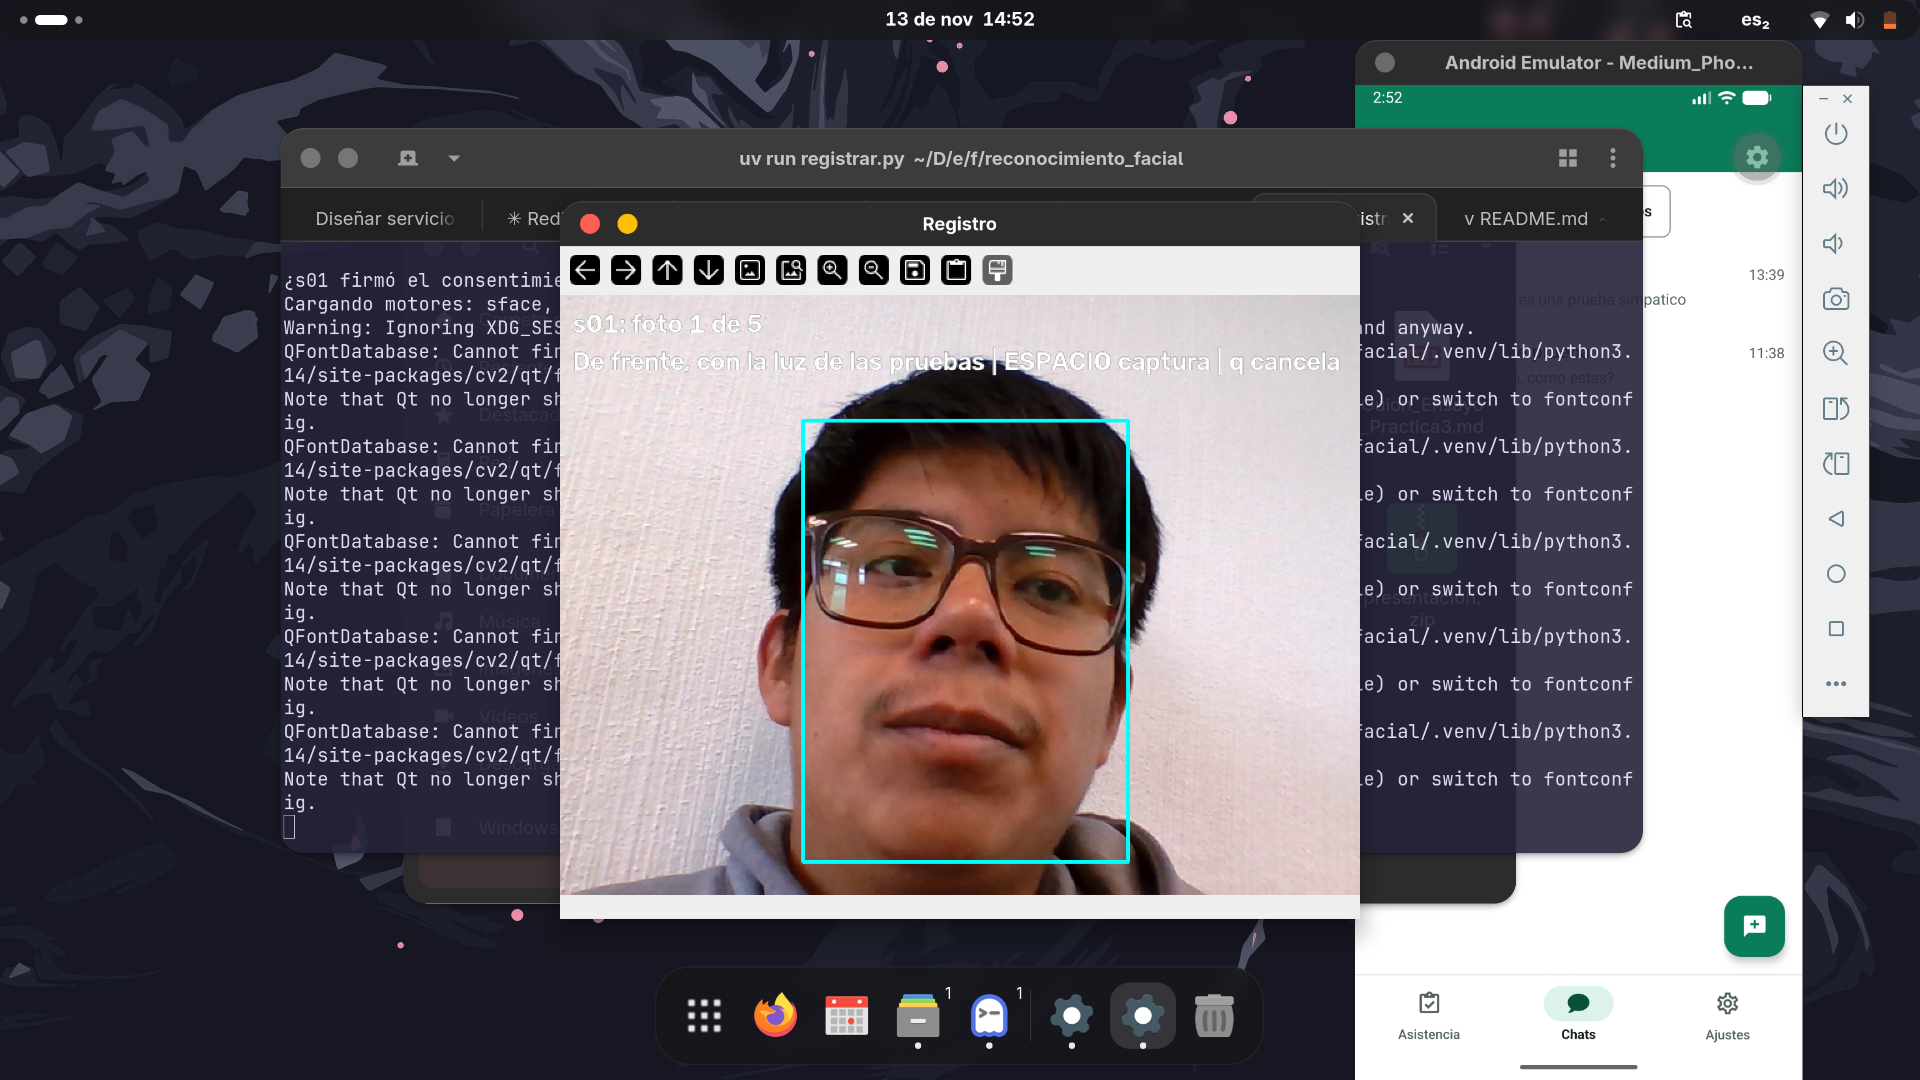
\includegraphics[width=\linewidth]{evidencias-2026-11-13/imagenes/01.png}
\end{center}
\figurenote{Captura del 13 de noviembre de 2026 a las 14:52:08. Se observa la ventana de registro, el encuadre de un rostro y la terminal del programa. La captura evidencia el procedimiento de registro; por sí sola no prueba que se hayan completado las cinco muestras ni que se hayan guardado todos los motores.}

El recuadro permite observar la detección del rostro durante el registro. La conclusión del proceso requiere verificar que se hayan guardado los vectores y asociado con el código del participante.

\clearpage
\subsection{Rechazo de una fotografía en un celular}
\begin{center}
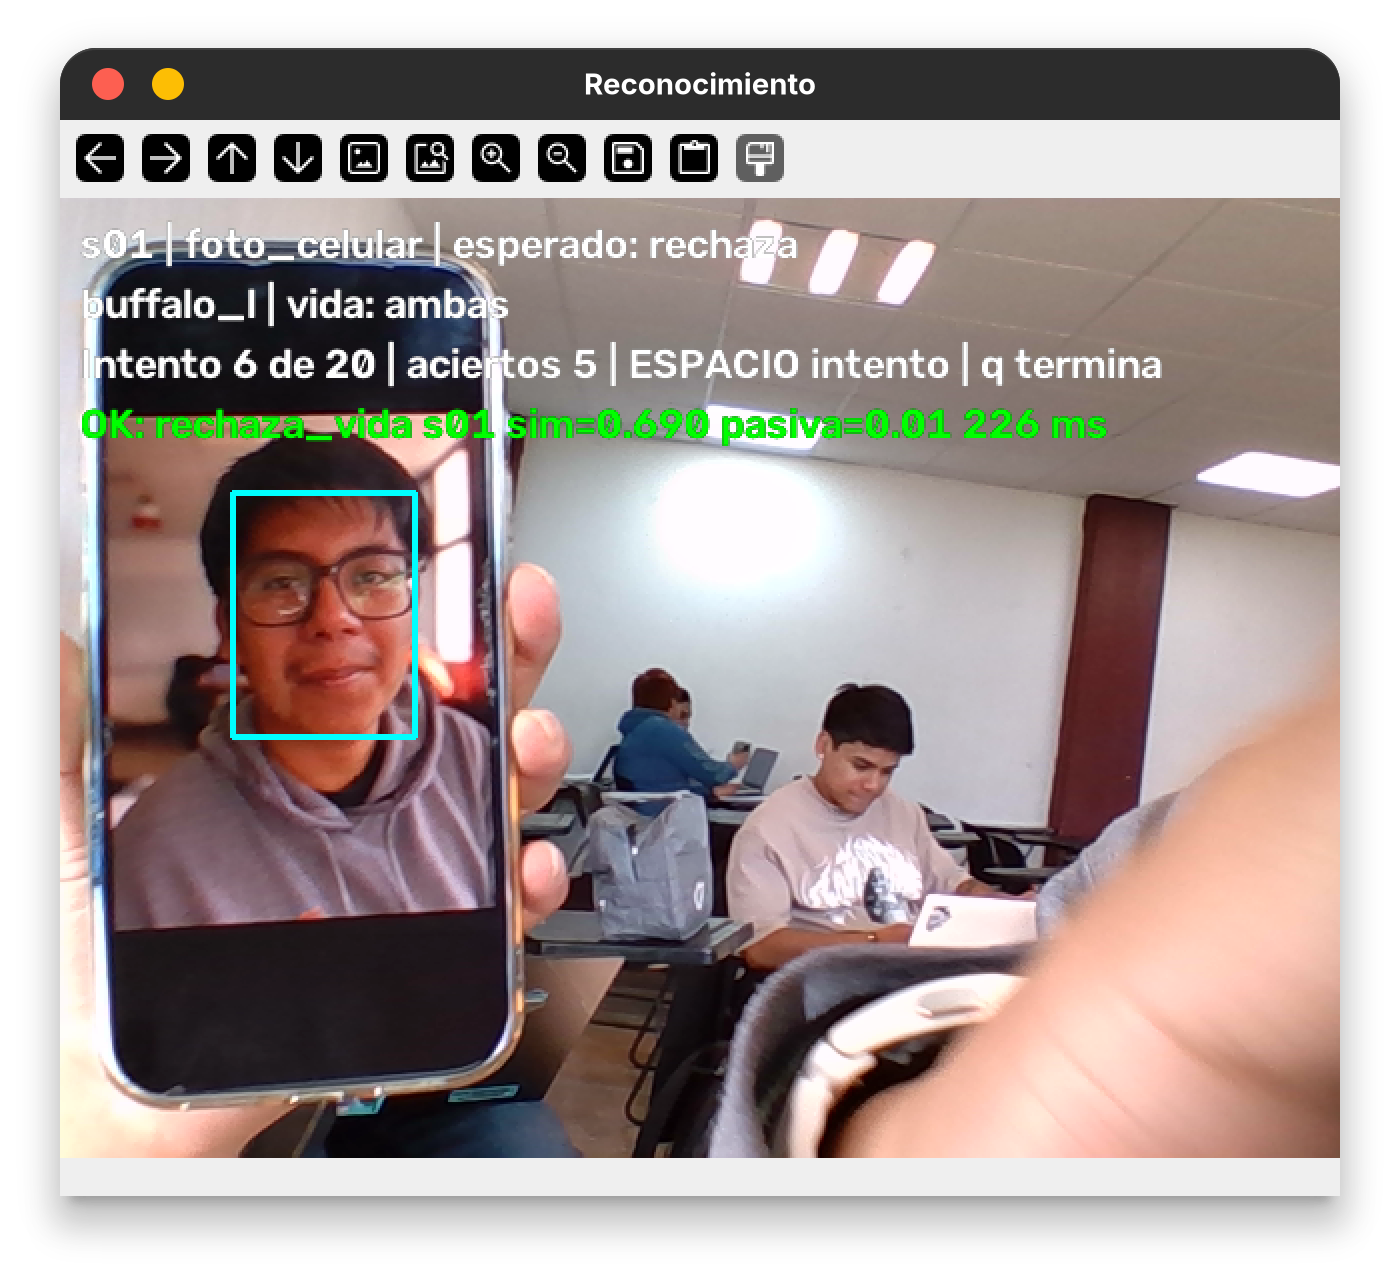
\includegraphics[height=16.5cm,width=\linewidth,keepaspectratio]{evidencias-2026-11-13/imagenes/02.png}
\end{center}
\figurenote{Captura del 13 de noviembre de 2026 a las 15:59:55. La pantalla indica s01, foto en celular, esperado rechazo y vida ambas. La última decisión visible es \texttt{rechaza\_vida}, similitud aproximada 0,690, puntaje pasivo 0,01 y 226 ms. Coincide con los valores del registro de las 15:59:39; la captura puede tomarse después de la decisión.}

Este resultado visual de rechazo debe leerse junto con los ocho intentos de la condición: el CSV también contiene la aceptación incorrecta de las 16:00:10. Una captura de éxito no sustituye el resumen completo.

\clearpage
\subsection{Aceptación con identidad distinta: primera captura}
\begin{center}
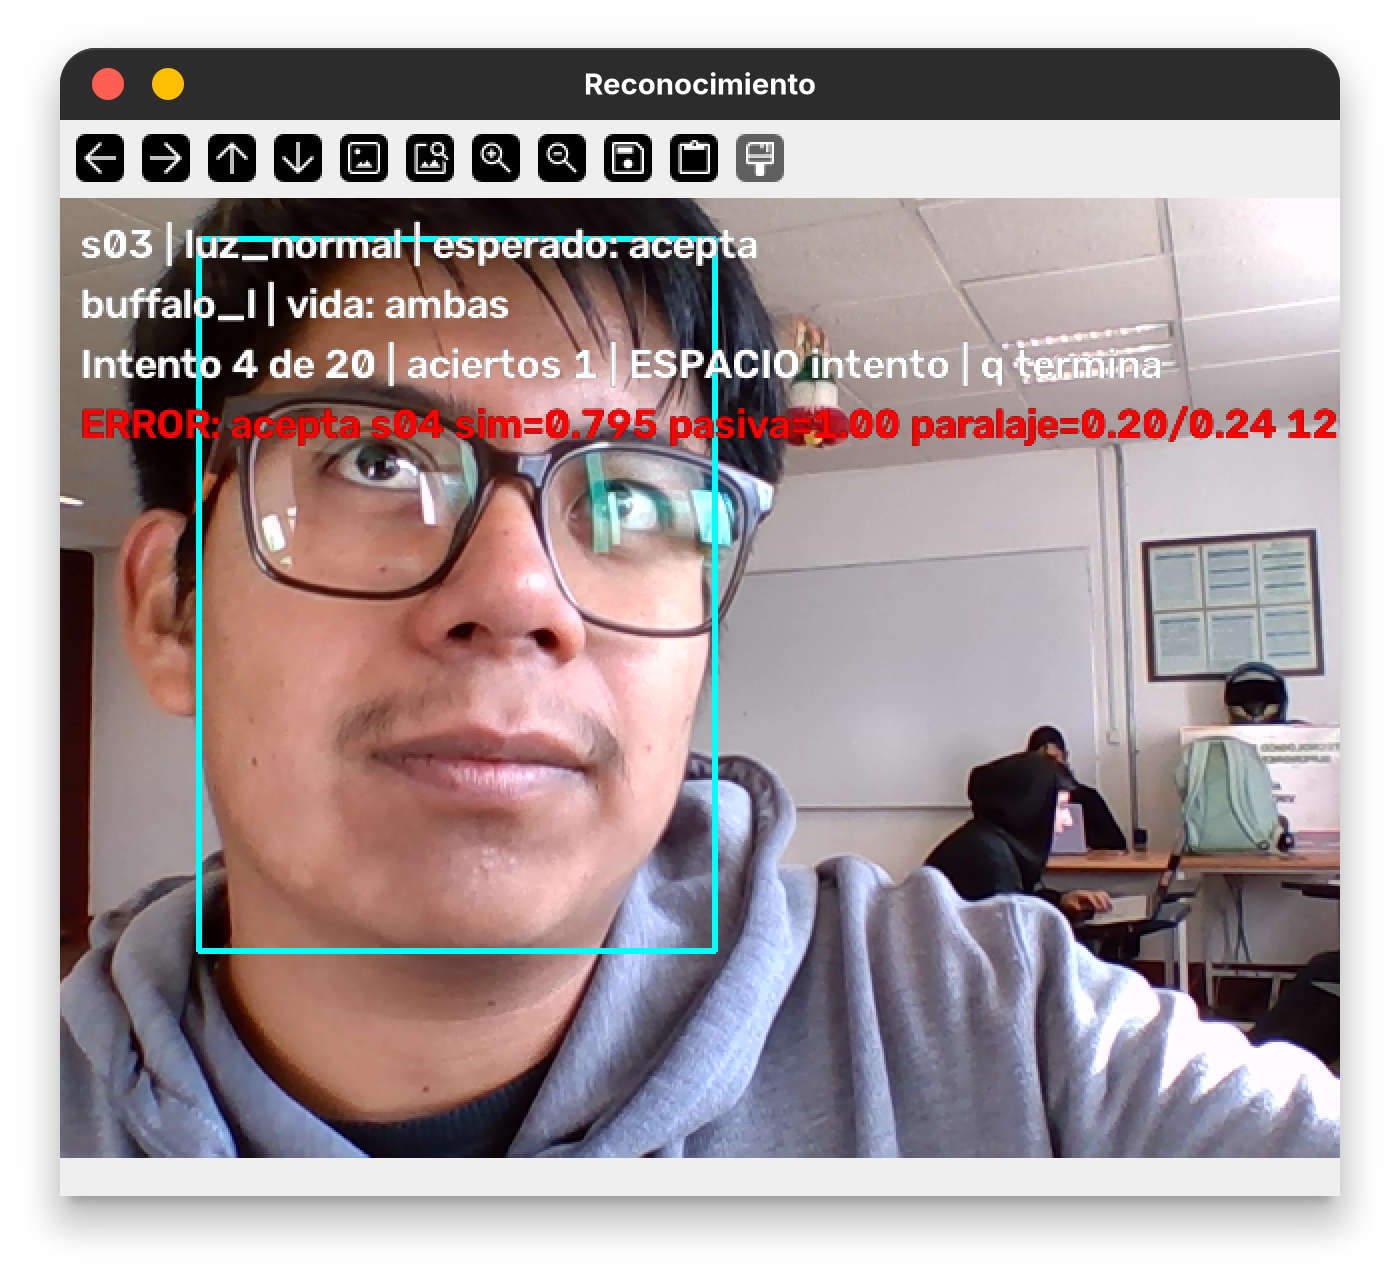
\includegraphics[height=16.5cm,width=\linewidth,keepaspectratio]{evidencias-2026-11-13/imagenes/03.png}
\end{center}
\figurenote{Captura del 13 de noviembre de 2026 a las 16:02:21. El encabezado indica s03 y esperado aceptación. En rojo, la interfaz conserva \texttt{ERROR: acepta s04}, similitud aproximada 0,795, vida pasiva 1,00 y paralaje 0,20/0,24. Es consistente con la decisión guardada a las 16:02:00.}

La prueba de vida no verifica que la etiqueta del participante sea correcta ni que el vector corresponda al código esperado. La revisión debe distinguir identificación, vida y etiquetado de sesión. Esta evidencia no determina por sí sola cuál de esos componentes originó la discrepancia.

\clearpage
\subsection{Aceptación con identidad distinta: segunda captura}
\begin{center}
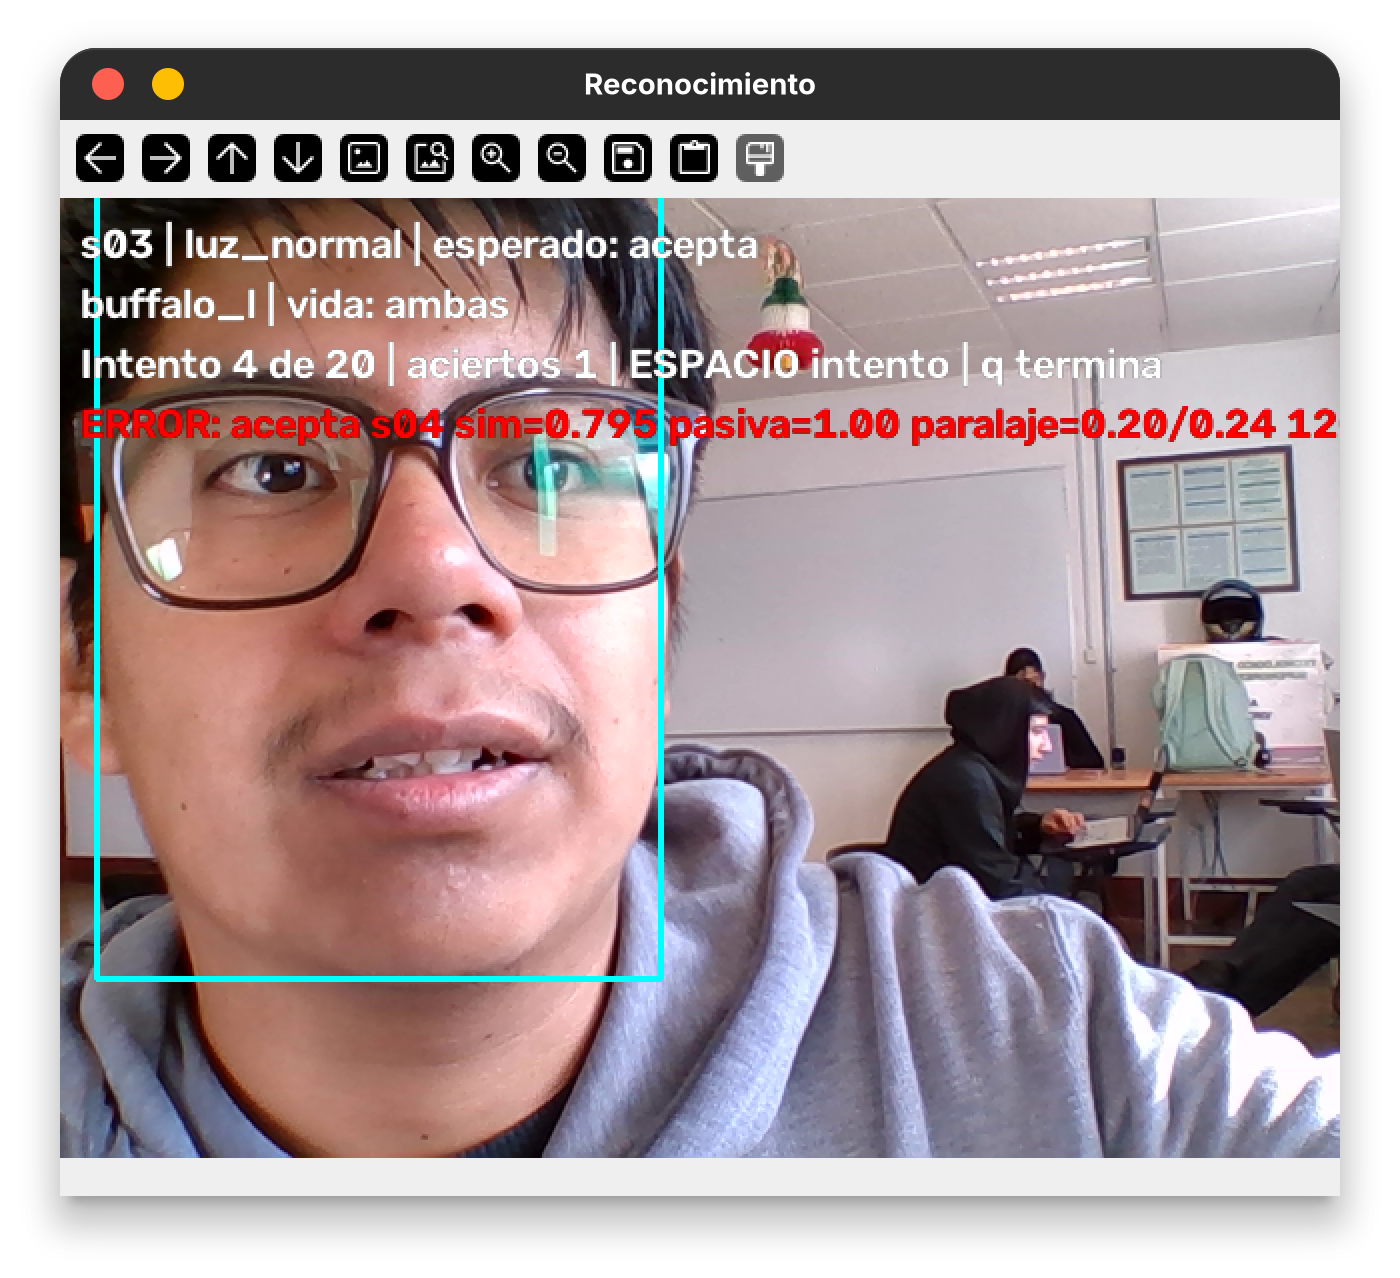
\includegraphics[height=16.5cm,width=\linewidth,keepaspectratio]{evidencias-2026-11-13/imagenes/04.png}
\end{center}
\figurenote{Captura del 13 de noviembre de 2026 a las 16:02:28. Conserva el encabezado de s03, el contador de intento 4 de 20 y la misma última decisión: aceptación como s04. Muestra que la última decisión permanece visible mientras continúa la vista de cámara, sin representar un intento adicional.}

Ambas capturas muestran el estado persistente de la interfaz entre intentos. Las repeticiones visibles de un resultado no se suman a los 24 registros; la marca de tiempo del CSV identifica el intento utilizado para el análisis.
